\documentclass{article}
\usepackage[a4paper, margin=3mm, landscape]{geometry}
\usepackage{multicol}
\usepackage{xcolor}
\usepackage{enumitem}
\usepackage{amsmath}
\usepackage{amsfonts}
\usepackage{listings}
\usepackage{soul}
\usepackage{graphicx}

\pdfinfo{
    /Title (CS4243.pdf)
    /Creator (TeX)
    /Producer (pdfTeX 1.40.0)
    /Author (Jason Qiu)
    /Subject (CS4243)
    /Keywords (CS4243, nus, cheatsheet, pdf)
}

\graphicspath{ {./img/} }

\pagestyle{empty}
\setcounter{secnumdepth}{0}
\setlength{\columnseprule}{0.25pt}

% Redefine section commands to use less space
\makeatletter
\renewcommand{\section}{\@startsection{section}{1}{0mm}%
    {-1ex plus -.5ex minus -.2ex}%
    {0.5ex plus .2ex}%x
{\normalfont\large\bfseries}}
\renewcommand{\subsection}{\@startsection{subsection}{2}{0mm}%
    {-1explus -.5ex minus -.2ex}%
    {0.5ex plus .2ex}%
{\normalfont\normalsize\bfseries}}
\renewcommand{\subsubsection}{\@startsection{subsubsection}{3}{0mm}%
    {-1ex plus -.5ex minus -.2ex}%
    {1ex plus .2ex}%
{\normalfont\small\bfseries}}%
\makeatother

% Adjust spacing for all itemize/enumerate
\setlength{\leftmargini}{0.5cm}
\setlength{\leftmarginii}{0.5cm}
\setlist[itemize]{leftmargin=2mm,labelindent=1mm,labelsep=1mm,label=$\bullet$}
\setlist[enumerate]{leftmargin=3mm,labelindent=1mm,labelsep=1mm,label=\arabic*.}

% Adjust column separator width in matrix
\setlength{\arraycolsep}{2.5pt}

% Font
\renewcommand{\familydefault}{\sfdefault}

% Define colors for math formulas
\definecolor{myblue}{cmyk}{1,.72,0,.38}
\everymath\expandafter{\the\everymath \color{myblue}}

% Custom command for keywords
\definecolor{highlight}{RGB}{251,243,218}
\newcommand{\keyword}[2]{\sethlcolor{highlight}\hl{\textbf{#1}} - #2}
\newcommand{\ilkeyword}[1]{\sethlcolor{highlight}\hl{\textbf{#1}}}

% Define colors and style for code
\definecolor{codegreen}{rgb}{0,0.6,0}
\definecolor{codegray}{rgb}{0.5,0.5,0.5}
\definecolor{codered}{HTML}{CC241D}
\definecolor{backcolor}{rgb}{0.95,0.95,0.95}
\lstdefinestyle{codestyle}{
    backgroundcolor = \color{backcolor},
    commentstyle = \color{codegray},
    keywordstyle = \color{codered},
    stringstyle = \color{codegreen},
    basicstyle = \ttfamily,
    breakatwhitespace = false,
    showstringspaces = false,
    breaklines = true,
    showtabs = false,
    tabsize = 2
}
\lstset{style = codestyle}

% -----------------------------------------------------------------------
\begin{document}
\begin{multicols*}{4}
\footnotesize

% Title box
\begin{center}
    \fbox{
        \parbox{0.8\linewidth}{
            \centering \textcolor{black}{
                {\Large\textbf{CS4243}} \\
                \normalsize{AY23/24 Sem 2}} \\
                {\footnotesize \textcolor{gray}{github.com/jasonqiu212}}
        }
    }
\end{center}

\section{01. Introduction}

\begin{itemize}
    \item $f(x,y) = i(x,y)r(x,y)$ where $f$ is intensity, $i$ is illumination, and $r$ is reflectance
    \item \keyword{Exposure time}{Time for incident light to reach sensor}
    \item \keyword{Storage}{$b = MNK$ where img. has size $M \times N$ and $K$-bit depth}
    \item Color to greyscale: $I = W_R R + W_G G + W_B B$ where $\sum_{i \in [R,G,B]} W_i = 1$
    \begin{itemize}
        \item Common weights: $(.299,.587,.114)$
    \end{itemize}
    \item \keyword{Norm. RGB}{$(r,g,b) = (\frac{R}{R+G+B},\frac{G}{R+G+B},\frac{B}{R+G+B})$}
    \item $(R,G,B) \leftrightarrow (r,g,b) \leftrightarrow (r,g,I)$ where $I = \frac{R+G+B}{3}$
    \item \ilkeyword{HSV Color Space}
    \begin{itemize}
        \item Hue: Pure color (0 to 360)
        \item Saturation: Mix pure color (1) with white light (0)
        \item Value: Mix from black (0) to white (255)
    \end{itemize}
\end{itemize}

\section{02. Filtering}

\begin{itemize}
    \item \keyword{Point processing}{$x_{ij} = f(p_{ij})$}
    \begin{itemize}
        \item \keyword{Brightness}{$x_{ij} = p_{ij} + b$ (Clipping behavior)}
        \item \keyword{Intensity scaling}{$x_{ij} = a p_{ij}$ (Increased/decreased contrast)}
        \item \keyword{Normalization (Whitening)}{$x_{ij} = \frac{p_{ij} - \mu}{\sigma}$ $\sigma^2 = \frac{\sum_{i = 0}^{I} \sum_{j = 0}^{J} (p_{ij} - \mu)^2}{IJ}$}
        \item \keyword{Gamma}{$x_{ij} = 255 (\frac{p_{ij}}{255})^\gamma$} where $\gamma > 0$
        \item \keyword{Intensity Histogram}{No data on location}
        \begin{itemize}
            \item \keyword{Stretching}{$x = (p - f_{\text{min}})(\frac{255}{f_{\text{max}} - f_{\text{min}}})$}
            \item \keyword{Equalization}{Turn cumulative distribution linear}
            \begin{enumerate}
                \item Get histogram: $h_k = \sum_{i = 0}^{I} \sum_{j = 0}^{J} \delta$ where $\delta = 1$ if $p_{ij} - k = 0$ and $0$ otherwise
                \item Estimate CDF: $c_k = \frac{\sum_{l = 1}^{k} h_l}{IJ}$
                \item Map $p_{ij} = k$ to new bin $x_{ij}$: $x_{ij} = 255 \text{CDF}(k)$
            \end{enumerate}
            \begin{itemize}
                \item Pros: More contrast than normalization, less prone to outliers than stretching
                \item Cons: More expensive
            \end{itemize}
            \item Good for foreground and background separation: Bi-modal histogram can be thresholded
            \item \keyword{Otsu's Method}{Automated thresholding}
            \begin{itemize}
                \item $T^* = \min_{T \in [0,255]} (w_1 (T) \sigma_1^2 (T) + w_2(T) \sigma_2^2 (T))$ where $T^*$ is the optimal threshold that min. sum of weighted variances of object and background
                \item $\sigma_1^2(T)$ and $\sigma_2^2(T)$: Variance of pixels less than or equal to and greater than threshold respectively
                \item $w_1(T)$ and $w_2(T)$: Number of pixels less than or equal to and greater than threshold
            \end{itemize}
        \end{itemize}
    \end{itemize}
    \item \keyword{Correlation Filtering}{Window (Moving average)}
    \begin{itemize}
        \item Motivation: Reduce noise
        \begin{itemize}
            \item Impulse noise: Random white occurrences of pixels
            \item Salt and pepper noise: Rand. white and black pixels
            \item Gaussian noise: Variations in intensity from Gaussian distribution $p_{ij} = \hat{p}_{ij} + \eta$ where $\eta \sim N(\mu_n, \sigma_n)$
        \end{itemize}
        \item $x_{ij} = \sum_{u=-k}^{k} \sum_{v=-k}^{k} f_{uv} \cdot p_{i+u,j+v}$ where $f$ is a \ilkeyword{kernel} of weights
        \item Notation: $X = P \otimes F$
        \item \keyword{Box Filter}{Blurs image}

        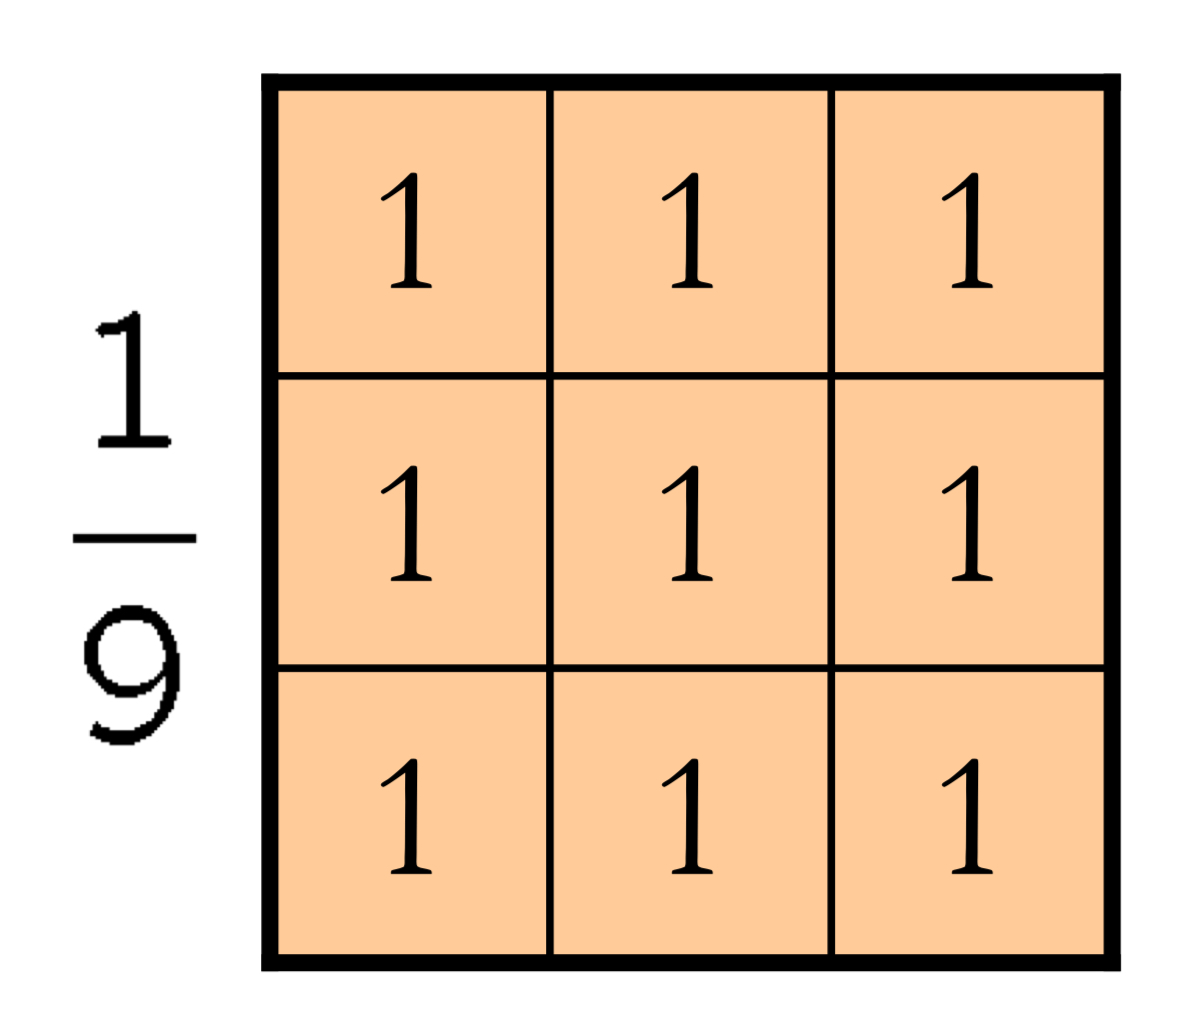
\includegraphics[scale=0.05]{box-filter.jpg}
        \item Given kernel of width $2k+1$, add padding: $\lfloor \frac{2k+1}{2} \rfloor$
        \begin{itemize}
            \item Filling methods: Zero-padding, wrap around, copy edge, reflect
        \end{itemize}
        \item \keyword{Gaussian Filter}{Nearest neighboring pixels have more weight}
        \begin{itemize}
            \item $f_{uv} = \frac{1}{2 \pi \sigma^2} e^{-\frac{u^2 + v^2}{2\sigma^2}}$

            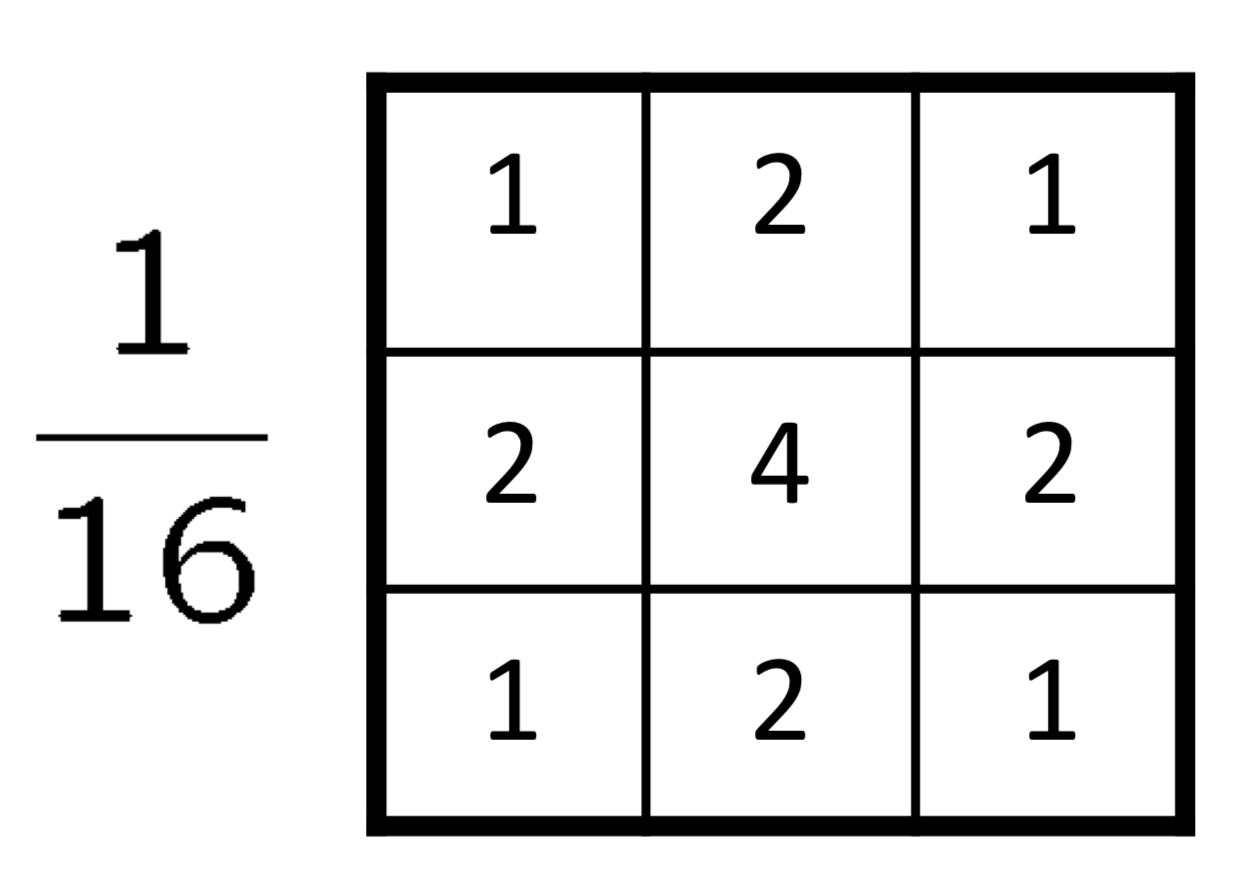
\includegraphics[scale=0.05]{gaussian-filter.jpg}
            \item Size of kernel: At some threshold, kernel will have lots of 0s, which is not useful
            \item Variance: Determines smoothing effect
        \end{itemize}
    \end{itemize}
    \item \keyword{Template Matching}{Set template as kernel and match occurs at local max.}
    \begin{itemize}
        \item \keyword{Normalized Cross-Correlation}{Normalizes using filter and input window}
        \begin{itemize}
            \item Motivation: Non-normalized is dominated by original image pixels
        \end{itemize}
        \item $x_{ij} = \frac{1}{|F||w_{ij}|} \sum_{u=-k}^{k} \sum_{v=-k}^{k} f_{uv} \cdot p_{i+u,j+v}$ where $|\cdot|$ is magnitude of kernel (i.e. Square root of sum of squares)
    \end{itemize}
    \item \keyword{Convolution Filtering}{Flip kernel in both directions, then do cross-correlation}
    \begin{itemize}
        \item $x_{ij} = \sum_{u=-k}^{k} \sum_{v=-k}^{k} f_{uv} \cdot p_{i-u,j-v}$
        \item Notation: $X = F * P$
        \item Convolution has nicer properties than correlation
        \item Properties: Commutative, Associative, Distributive over addition, Scalar factor, Identity
    \end{itemize}
    \item \keyword{Non-Linear Filters}{Filters that perform non-linear operations (e.g. Median, Min., Max.)}
    \begin{itemize}
        \item Correlation and convolution are both linear operations
        \item \ilkeyword{Median Filtering}
        \begin{itemize}
            \item Removes spikes: Good for removing impulse and salt and pepper noise
            \item No new pixel values introduced
            \item Edge preserving
        \end{itemize}
    \end{itemize}
\end{itemize}

\section{03. Gradients}

\section{04. Lines}

\begin{itemize}
    \item Goal: Which points belong to which line?
    \item $y = mx + b$ $\quad$ $\frac{x}{a} + \frac{y}{b} = 1$
    \item $x \cos \theta + y \sin \theta = \rho$
    \item \keyword{Line fitting}{$E = \frac{1}{N} \sum_i (y_i - (mx_i + b))^2$}
    \begin{itemize}
        \item Goal: Find parameters $m$ and $b$ that min. $E$
        \item Using gradient descent: $b = \bar{y} - m\bar{x}$ $\quad$ $m = \frac{\sum_i (x_i - \bar{x})(y_i - \bar{y})}{\sum_i (x_i - \bar{x})^2}$ where $\bar{y} = \frac{\sum_i y_i}{N}$ and $\bar{x} = \frac{\sum_i x_i}{N}$
        \item Cons: Choice of error function, outliers
    \end{itemize}
    \item \keyword{Hough Transform}{Paramterize shape and vote}
    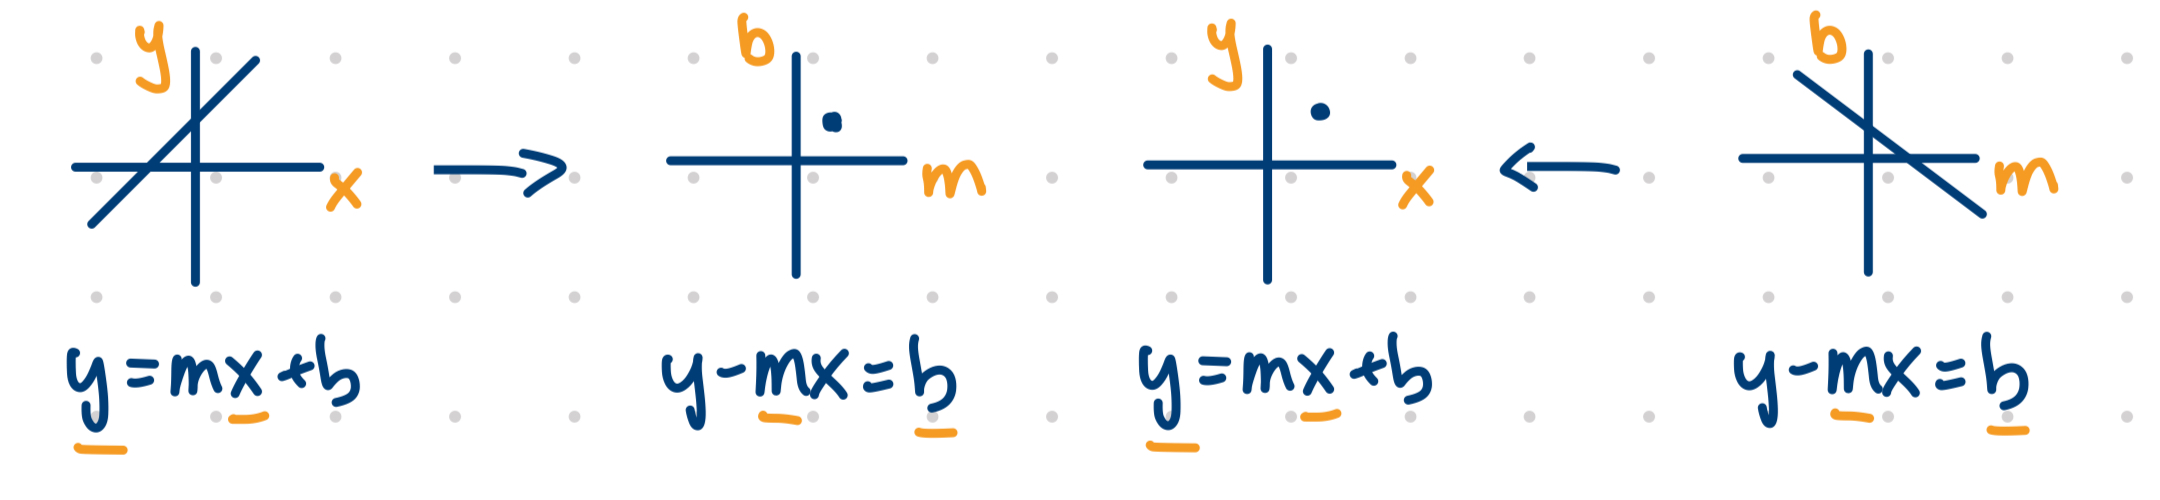
\includegraphics[scale=0.089]{line-paramterization.jpg}
    \begin{enumerate}
        \item Initialize accumulator array $A(\theta, \rho) = 0$
        \item For each image edge point $(x_i, y_i)$:
        \begin{enumerate}
            \item For each $\theta$:
            \begin{enumerate}
                \item Solve for $\rho = x_i \cos \theta + y_i \sin \theta$
                \item $A(\theta, \rho) = A(\theta, \rho) + 1$
            \end{enumerate}
        \end{enumerate}
        \item Find maximum in $A(\theta, \rho)$
        \item Detected lines are given by $\rho^* = x\cos\theta^* + y\sin\theta^*$
    \end{enumerate}
    \item \keyword{Circle}{$(x-a)^2 + (y-b)^2 = r^2$}
    \begin{itemize}
        \item If $r$ is unknown, need to solve for 3 parameters (i.e. $A(a,b) \rightarrow A(a,b,r)$) and a point becomes a cone in 3D parameter space
        \item Optimization: Use gradient
        \begin{itemize}
            \item Use edge orientation $\phi_i$ to vote for 2 points, rather than whole circle
        \end{itemize}
    \end{itemize}
    \item \keyword{Generalized Hough Transform}{Arbitrary shape}
    \begin{enumerate}
        \item Given shape with boundary points $p_i$ and reference point $a$
        \item For each $p_i$, get displacement vector from $a$
        \item Store in table with key $\phi_i$ and value (Displacement vectors)
        \item For each edge pt., use $\phi_i$ to get vectors to vote for $a$
    \end{enumerate}
    \begin{itemize}
        \item Application: Index with local pattern, instead of gradients
        \item Tips: Soft voting, convert to edge image
        \item Pros: Food with noise and occlusion
        \item Cons: Complexity with num. of parameters, grid size
    \end{itemize}
\end{itemize}

\section{05. Segmentation}

\begin{itemize}
    \item Goal: Separate image into coherent regions
    \item Idea: \keyword{Clustering}{Group similar data points together}
    \item Challenges: What makes 2 points same/different? Choice of features (e.g. Color, Intensity, Position), Which clustering algorithm?
    \item \keyword{k-Means Clustering}{Iteratively re-assign points to nearest cluster center}
    \begin{enumerate}
        \item Randomly initialize the cluster centers $c_1, \ldots, c_K$
        \item For each point $p_i$, find the closest $c_j$ to put $p_i$ in
        \item Set $c_j$ to be mean of points in cluster $j$
        \item Repeat, if $c_j$ have changed up to some threshold
    \end{enumerate}
    \begin{itemize}
        \item Pros: Simple, Converges to local min.
        \item Cons: Setting $K$, Sensitive to initial centers (Since k-means converges to local min.), Sensitive to outliers (Can add more clusters), Assumes spherical clusters
    \end{itemize}
    \item \ilkeyword{Simple Linear Iterative Clustering (SLIC) Superpixels}
    \begin{itemize}
        \item \keyword{Superpixel}{Group of pixels that share common traits}
        \begin{itemize}
            \item Application: Inputs to other CV algo. since more compact representation with perceptual meaning
        \end{itemize}
        \item Num. of pixels: $n_{tp}$; Target num. of superpixels: $n_{sp}$
        \item Initial width of each superpixel: $s = \sqrt{n_{tp} / n_{sp}}$
        \item Features: $z = [r,g,b,x,y]$
        \item Color distance: $d_c = || \langle r_j,g_j,b_j \rangle - \langle r_i,g_i,b_i \rangle ||$
        \item Spatial distance: $d_s = || \langle x_j,y_j \rangle - \langle x_i,y_i \rangle ||$
        \item Scaling factors: $d_{cm}$ and $d_{sm}=s$ set as max. expected values of $d_c$ and $d_s$ respectively
        \item $D = \sqrt{(\frac{d_c}{d_{cm}})^2+(\frac{d_s}{d_{sm}})^2} = \sqrt{d_c^2 + (\frac{d_s}{s})^2 c^2}$
    \end{itemize}
    \begin{enumerate}
        \item Split img. into grid of size $s \times s$. Set cluster centers as lowest gradient position in $3 \times 3$ neighborhood from superpixel center to speed up convergence since initialize on value common to surrounding.
        \item For each cluster center, check distance to all pixels within $2s \times 2s$ neighborhood. Assign pixels to closest checked center.
        \item Update cluster centers using mean and repeat if not converged (Same as k-Means)
        \item Optional: Replace superpixel region by average value to create stained glass effect
    \end{enumerate}
    \begin{itemize}
        \item Modification of k-Means: Not random initialization, Compute pixel's distance only to closest set of cluster centers
    \end{itemize}
    \item \keyword{Mean-Shift Clustering}{Find local density maxima in feature space}
    \begin{itemize}
        \item \keyword{Attraction basin}{Region in feature space for which all trajectories of centroids lead to same mode}
        \item \keyword{Cluster}{All data points in attraction basin of a mode}
    \end{itemize}
    \begin{enumerate}
        \item For each data point:
        \begin{enumerate}
            \item Define window around and get centroid
            \item Shift window to centroid
            \item Repeat until window centroid stops moving
        \end{enumerate}
    \end{enumerate}
    \begin{itemize}
        \item Segmentation with Mean Shift: Do mean shift and merge pixels in same attraction basin
        \item Choosing window size: Trial and error, Sample points and use avg. dist. to knn. (Num. of neighbors needs to be large enough to ensure increase in density)
        \begin{itemize}
            \item Larger window size $\rightarrow$ Fewer clusters
        \end{itemize}
        \item Pros: No assumptions on cluster shape, 1 parameter, Finds variable num. of modes (vs. specified $k$ in k-Means), Robust to outliers
        \item Cons: Choosing $h$, Slow, Scales poorly with feature space dimension
        \item Optimizations:
        \begin{itemize}
            \item After each run of mean shift, assign all points within radius $r$ of end point to same cluster
            \item Assign points in radius $c < r$ of search path to mode
        \end{itemize}
    \end{itemize}
\end{itemize}

\end{multicols*}
\end{document}
